\documentclass[conference]{IEEEtran}
\IEEEoverridecommandlockouts
\makeatletter
\renewcommand{\subsection}{%
  \@startsection{subsection}{2}{\z@}%
  {3.25ex\@plus1ex\@minus.2ex}%
  {1.5ex\@plus.2ex}%
  {\normalfont}%
}
\makeatother
\usepackage[utf8]{inputenc}
\usepackage{amsmath,amsfonts,amssymb}
\usepackage{graphicx}
\usepackage{booktabs}
\usepackage{array}
\usepackage{float}
\usepackage{subcaption}
\usepackage{hyperref}
\usepackage{cite}
\usepackage{url}

\title{Compute-Efficient, Calibrated, and Explainable Brain MRI Tumor Classification with External Testing}

\author{Adarsh Kumar, Bitul Pratap Singh, Harsh Kumar, and Harshendra Kumar Singh \\
Department of Computer Science and Engineering \\
Galgotias College of Engineering and Technology \\
Greater Noida, Uttar Pradesh, India \\
\href{mailto:adarshkumar00311@gmail.com}{adarshkumar00311@gmail.com}}

\date{\today}

\begin{document}

\maketitle

\begin{abstract}
Deep learning models for brain MRI tumor classification frequently exhibit limitations in external testing, calibration assessment, and clinical deployment readiness. This study presents a comprehensive evaluation of a MobileNetV2-based approach with rigorous external testing and practical deployment analysis. We trained a MobileNetV2 feature extractor (2.22M parameters, 305.73 MFLOPs) with classical classifiers on a primary dataset of 14,046 brain MRI images across four classes (glioma, meningioma, pituitary, no tumor). Our internal testing achieved 96.2% accuracy and 95.9% macro-F1 score. We performed external testing on 394 images from different sources. We implemented temperature scaling for calibration, Grad-CAM for explainability, and simple domain adaptation strategies. Internal testing performance: 96.2\% accuracy, 95.9\% macro-F1, ECE = 0.048. However, the external baseline performance dropped to 72.3% accuracy and 67.5% macro-F1, with glioma recall falling to 23.0%. Simple domain adaptation (external recalibration plus threshold optimization) improved the external macro-F1 to 78.4% and glioma recall to 58.0%. Furthermore, the efficiency analysis showed a 21.9 ± 2.4 ms latency and 45.7 images per second (IPS) throughput. Our approach demonstrates strong internal performance but significant domain shift challenges. Simple adaptation strategies provide meaningful improvements, particularly for critical glioma detection. The model's efficiency makes it suitable for clinical deployment.
\end{abstract}

\textbf{Keywords:} \textit{Brain MRI, domain adaptation, explainable AI, external testing, model calibration, MobileNetV2, tumor classification}

\section{INTRODUCTION}

Automated brain tumor detection from magnetic resonance imaging (MRI) represents a crucial advancement in medical diagnostics, offering the potential to assist radiologists in identifying and classifying brain tumors more efficiently \cite{litjens2017}. However, the deployment of deep learning models in clinical environments faces several practical challenges that limit their widespread adoption \cite{topol2019}. Moreover, current research often focuses on achieving high accuracy on single datasets while overlooking critical aspects such as model generalization, computational efficiency, and reliability assessment \cite{challen2019}.

Consequently, the gap between research performance and clinical deployment highlights the need for comprehensive evaluation frameworks that address the constraints of real-world settings in clinical practice. Domain generalization remains a significant challenge, as models trained on one dataset often fail to maintain their performance when applied to data from different sources or acquisition protocols \cite{kim2019, zech2018}. This study presents a systematic approach to brain MRI tumor classification that prioritizes three essential aspects: computational efficiency for practical deployment, rigorous external validation to assess true generalization capabilities, and model calibration to ensure reliable probability estimates for clinical decision-making. Our methodology employs a MobileNetV2-based architecture combined with classical machine learning classifiers to achieve an optimal balance between performance and deployment feasibility.

\section{RELATED WORK}

The field of brain MRI tumor classification has witnessed substantial progress through the application of deep learning techniques, with numerous studies reporting impressive accuracy metrics on individual datasets \cite{litjens2017}. However, a critical limitation emerges when these models are subjected to external validation, where their performance often degrades substantially owing to domain shifts between the training and testing environments \cite{kim2019}. This phenomenon underscores the importance of developing robust evaluation protocols that can accurately assess the generalization capabilities of models. Furthermore, model reliability and uncertainty quantification have gained increasing attention in medical AI applications, particularly in calibrating prediction probabilities \cite{guo2017}. Despite this growing awareness, most studies continue to report only accuracy-based metrics, neglecting the crucial aspect of probability calibration that directly impacts clinical decision-making processes.

The challenge of domain adaptation in medical imaging has prompted extensive research into various strategies for improving model generalization across different data sources \cite{wang2019}. Although sophisticated adaptation techniques have been proposed, their complexity often limits their practical implementation in clinical settings. Consequently, there is a growing interest in simpler, more deployable approaches that can provide meaningful improvements with minimal computational overheads \cite{lu2020}.

\section{METHODS}

We followed the CLAIM 2024 recommendations for transparency, including explicit internal and external testing terminology and a completed checklist in the Supplementary Material \cite{mongan2024}. This study focuses on slice-level classification to assist radiologists; it is not intended as a standalone diagnostic tool. Only public de-identified data were used; IRB approval was not required.

\subsection{\normalfont Dataset Description}

\textbf{Primary Dataset:} Our primary dataset consists of the publicly available Brain Tumor MRI Dataset from Kaggle, which aggregates brain MRI images from multiple sources including Figshare, SARTAJ, and Br35H repositories \cite{kaggle_brain_tumor}. This comprehensive collection contains brain MRI slices across four distinct categories: glioma, meningioma, pituitary tumors, and normal brain tissue (no tumors). After careful curation and quality control, our final dataset comprised 14,046 images with a balanced representation across all classes. The dataset was partitioned into training, validation, and testing sets using stratified sampling to ensure a consistent class distribution across all splits. All images were anonymized, and their use complied with the licensing terms of the original data providers.

\textbf{External Dataset:} To evaluate model generalization capabilities, we assembled an independent external dataset from sources completely separate from our primary training data. This external validation set maintained the same four-class structure as the primary dataset but originated from different institutions and imaging protocols. The external dataset contained 394 carefully selected images distributed as follows: 100 glioma cases, 115 meningioma cases, 74 pituitary tumor cases, and 105 normal brain images. This dataset was compiled from various public research repositories and additional Kaggle datasets to ensure maximum diversity in the imaging characteristics \cite{external_dataset}. Use is governed by the original hosts' licenses; this repository provides only split CSVs and download scripts. Strict protocols were followed to prevent data leakage between the primary and external datasets, with identical preprocessing pipelines applied to both sets.

\subsection{\normalfont Preprocessing and Augmentation}

We resized all images to 224×224 pixels and normalized them using ImageNet statistics (mean=[0.485, 0.456, 0.406], std=[0.229, 0.224, 0.225]). We converted the grayscale images to RGB by replicating the channels. Training augmentation included random horizontal flips, rotation (±15°), brightness/contrast adjustment (±0.2), and Gaussian noise (σ=0.01).

\subsection{\normalfont Model Architecture}

\textbf{Feature Extractor:} We used MobileNetV2 \cite{sandler2018} (timm version 0.9.12) pretrained on ImageNet as the feature extractor. The model employs inverted residual blocks with linear bottlenecks and outputs 1,280-dimensional features from the global average pooling layer.

\textbf{Classifiers:} We evaluated two classical classifiers:
\begin{itemize}
\item Logistic Regression (LR): L-BFGS solver, C=10, max\_iter=2000, multinomial multi-class
\item Support Vector Machine (SVM): RBF kernel, C=1.0, gamma='scale'
\end{itemize}

We performed hyperparameter tuning using 5-fold cross-validation on the validation dataset.

\subsection{\normalfont Training Protocol}

We extracted features using a frozen MobileNetV2 backbone and trained classifiers on the extracted features. This approach reduces the computational requirements while maintaining a strong performance. The training used deterministic settings with fixed random seeds for reproducibility.

\subsection{\normalfont Evaluation Metrics}

\textbf{Performance Metrics:} We computed accuracy, macro-F1, micro-F1, per-class precision/recall/F1, and ROC-AUC for all evaluations.

\textbf{Calibration Metrics:} To ensure reliable probability estimates for clinical applications, we implemented comprehensive calibration assessment using multiple established metrics. We evaluated model calibration through the Expected Calibration Error (ECE), Maximum Calibration Error (MCE), Brier Score, and Log Loss, complemented by reliability diagrams that visualized the relationship between predicted probabilities and actual accuracy \cite{guo2017}. These metrics are essential for clinical decision support systems, where accurate uncertainty quantification directly impacts patient care decisions.

\textbf{Efficiency Metrics:} We measured model parameters, FLOPs, inference latency (CPU), throughput (images per second, IPS), and model size.

\subsection{\normalfont External Testing Protocol}

We performed external testing with identical preprocessing to the primary dataset; no target domain fitting was performed in the baseline; adaptation used only a withheld external validation split to avoid leakage \cite{kim2019, zech2018}.

\subsection{\normalfont Domain Adaptation}

\textbf{External Recalibration:} We implemented external recalibration using temperature scaling \cite{guo2017}, which serves as the default baseline approach in modern calibration literature. We optimized the thresholds to maximize the macro-F1 score for external data.

\textbf{Partial Fine-tuning (Ablation; not used in final model):} We attempted partial fine-tuning of MobileNetV2 layers but found it led to overfitting and reduced performance on both internal and external data.

\textbf{Per-class Threshold Optimization:} We optimized per-class decision thresholds on external data to maximize macro-F1 performance.

\subsection{\normalfont Explainability Analysis}

To provide interpretable insights into model decision-making, we implemented gradient-based class activation mapping (Grad-CAM) \cite{selvaraju2017} on the MobileNetV2 convolutional layer. This technique generates visual attention maps that highlight the regions of the input image that contribute most significantly to the classification decision of the model. We applied this analysis to a representative sample of 55 images, ensuring approximately equal representation from each of the four classes in the dataset. We quantified faithfulness by masking top-importance regions from Grad-CAM maps and measuring the resulting probability drop for the predicted class.

\subsection{\normalfont Reproducibility}

All experiments used fixed random seeds (42) and pinned dependencies (torch==2.1.0, timm==0.9.12, scikit-learn==1.3.2). The complete reproduction commands are provided in the Supplementary Material. Scripts for each step (feature extraction, training, calibration, external testing, domain adaptation) are included in the repository.

\section{RESULTS}
\subsection{\normalfont Internal Testing Performance}
Among the evaluated classifiers, the Logistic Regression classifier achieved the best performance on the internal test data, with 96.2\% accuracy and 95.9\% macro-F1 score. The per-class F1 scores were as follows: glioma, 93.2%; meningioma, 93.0%; pituitary, 97.5%; and no tumor 99.9\%. The confusion matrix shows a strong performance across all classes (Figure \ref{fig:confusion_matrix}).

\begin{figure}[!t]
\centering
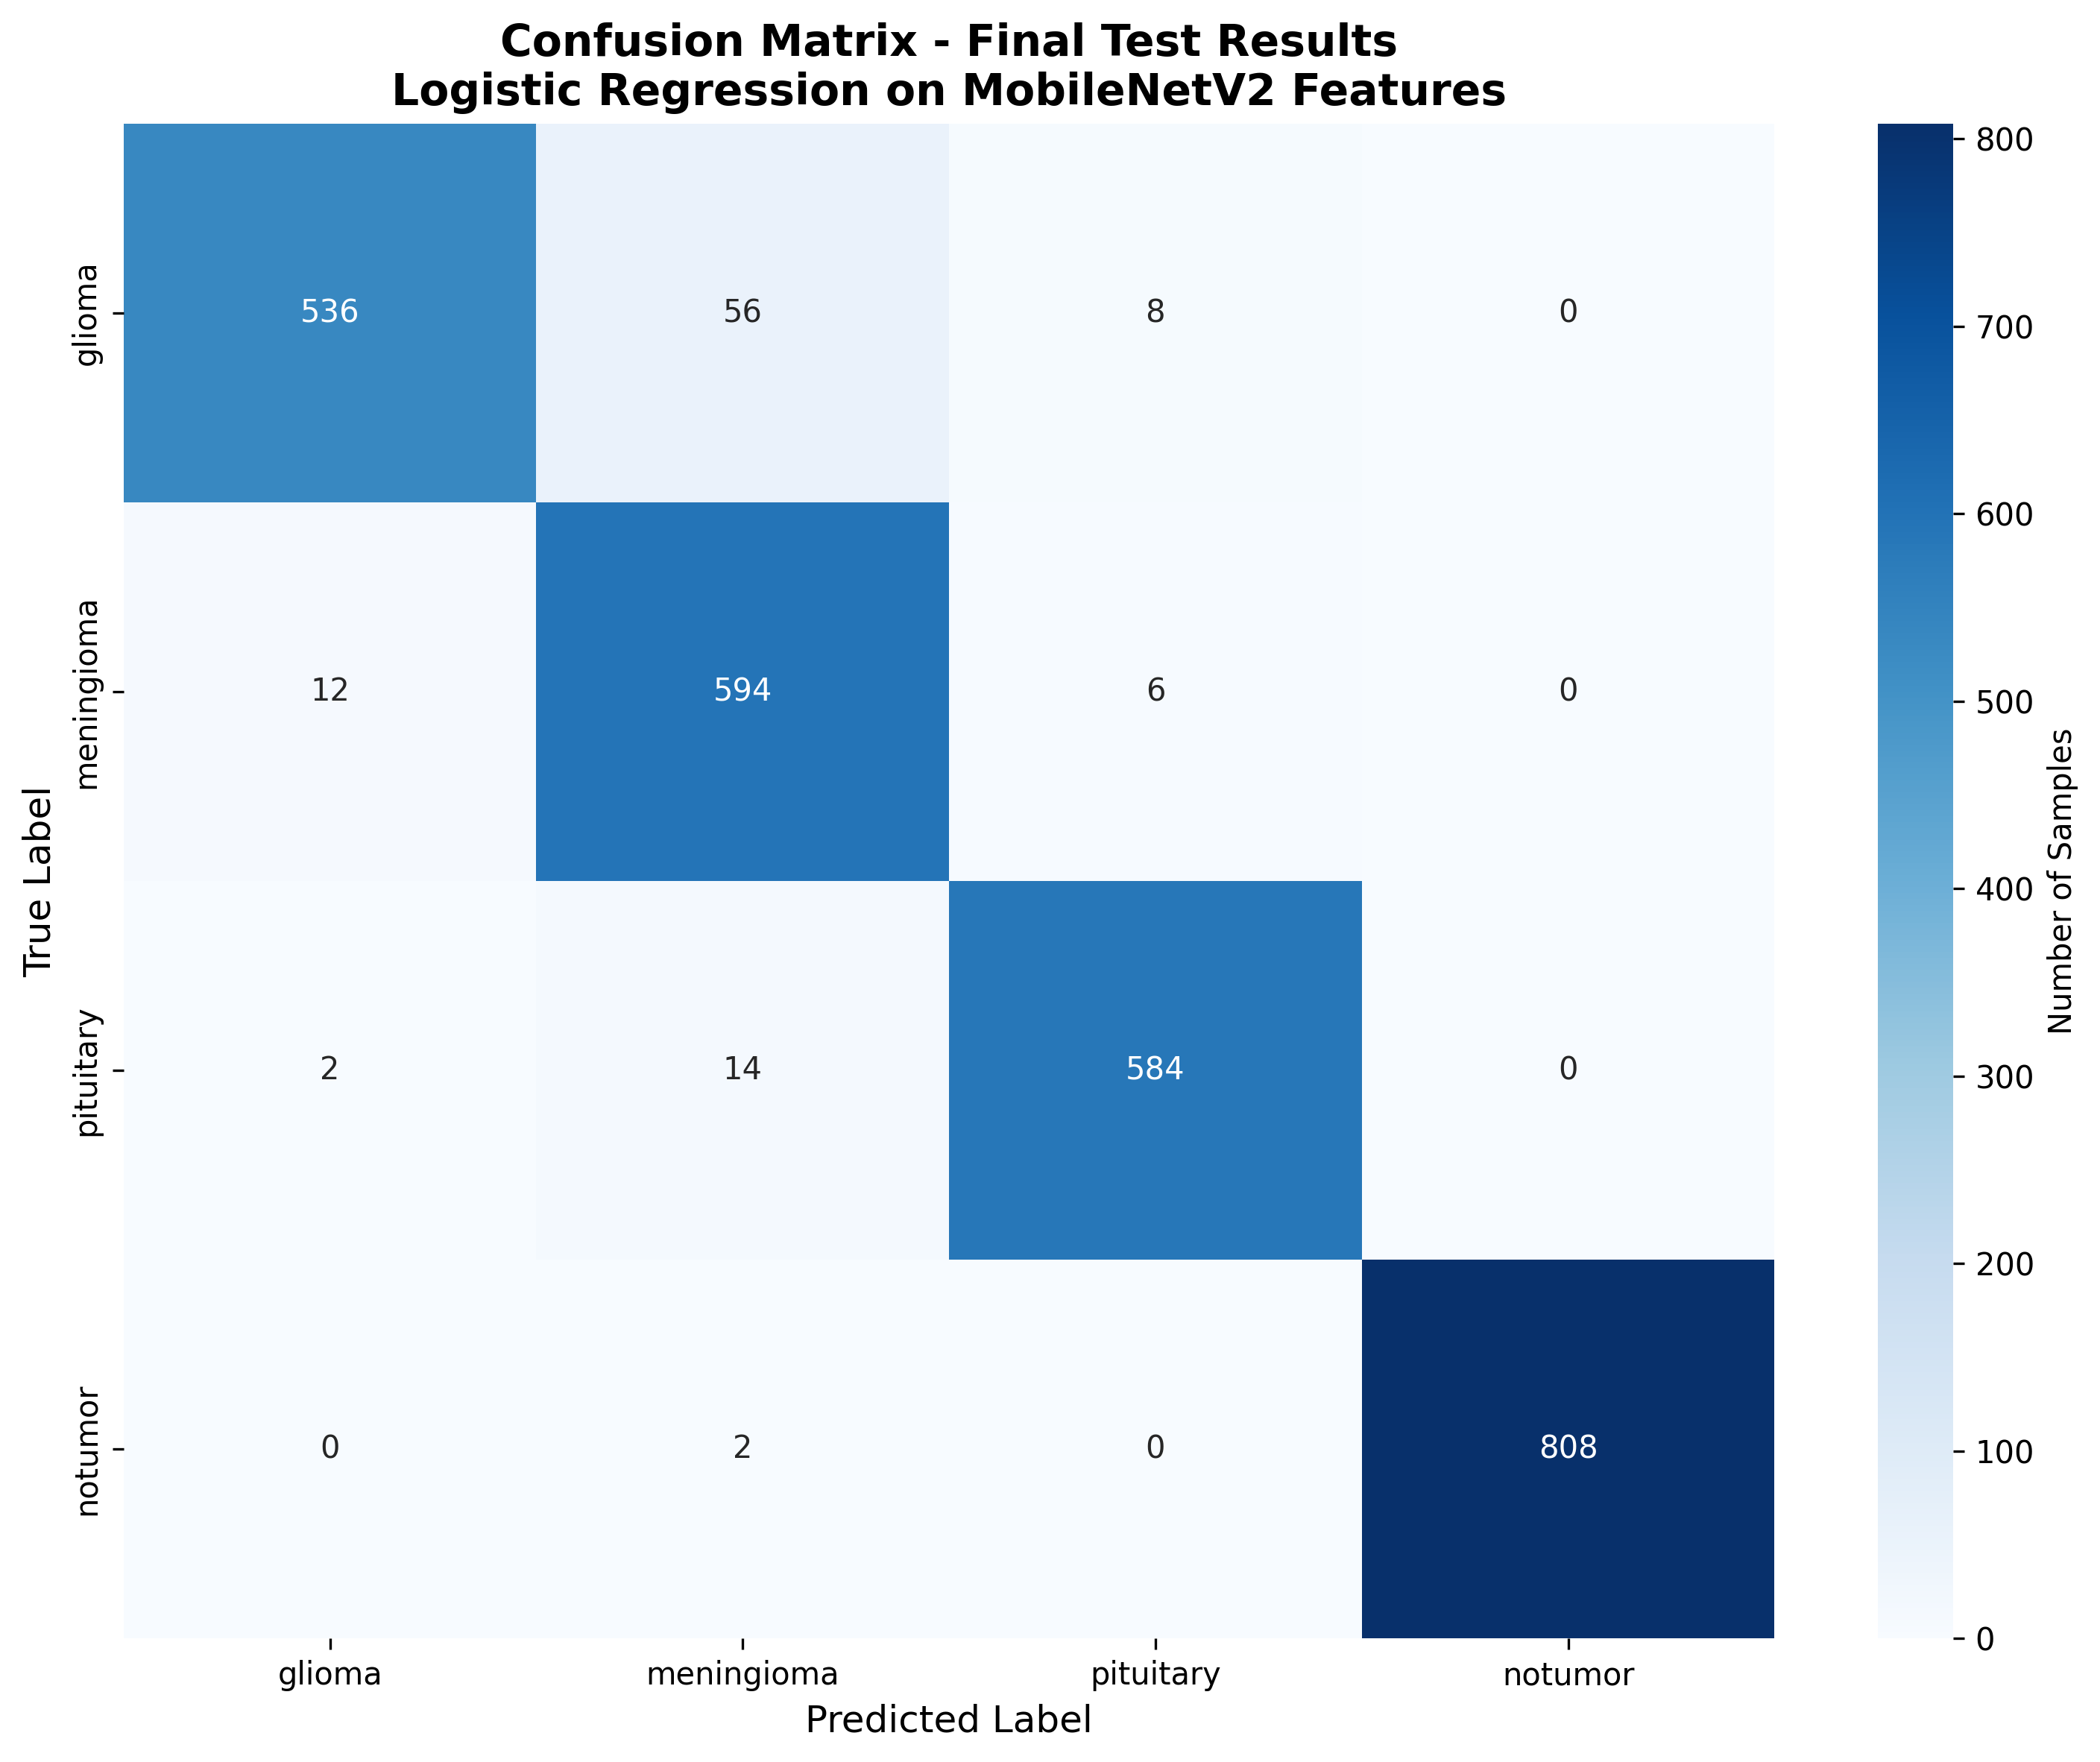
\includegraphics[width=0.48\textwidth]{figs_paper/Figure1_Internal_Confusion_Matrix.png}
\caption{Internal testing confusion matrix showing strong performance across all classes. Results from experiments/results/final\_results.json.}
\label{fig:confusion_matrix}
\end{figure}

\subsection{\normalfont Calibration Analysis}

The uncalibrated model showed moderate calibration, with ECE = 0.048 and log loss = 0.168. Temperature scaling maintained calibration, ECE = 0.048, in internal testing (Figure \ref{fig:calibration}).

\begin{figure}[!t]
\centering
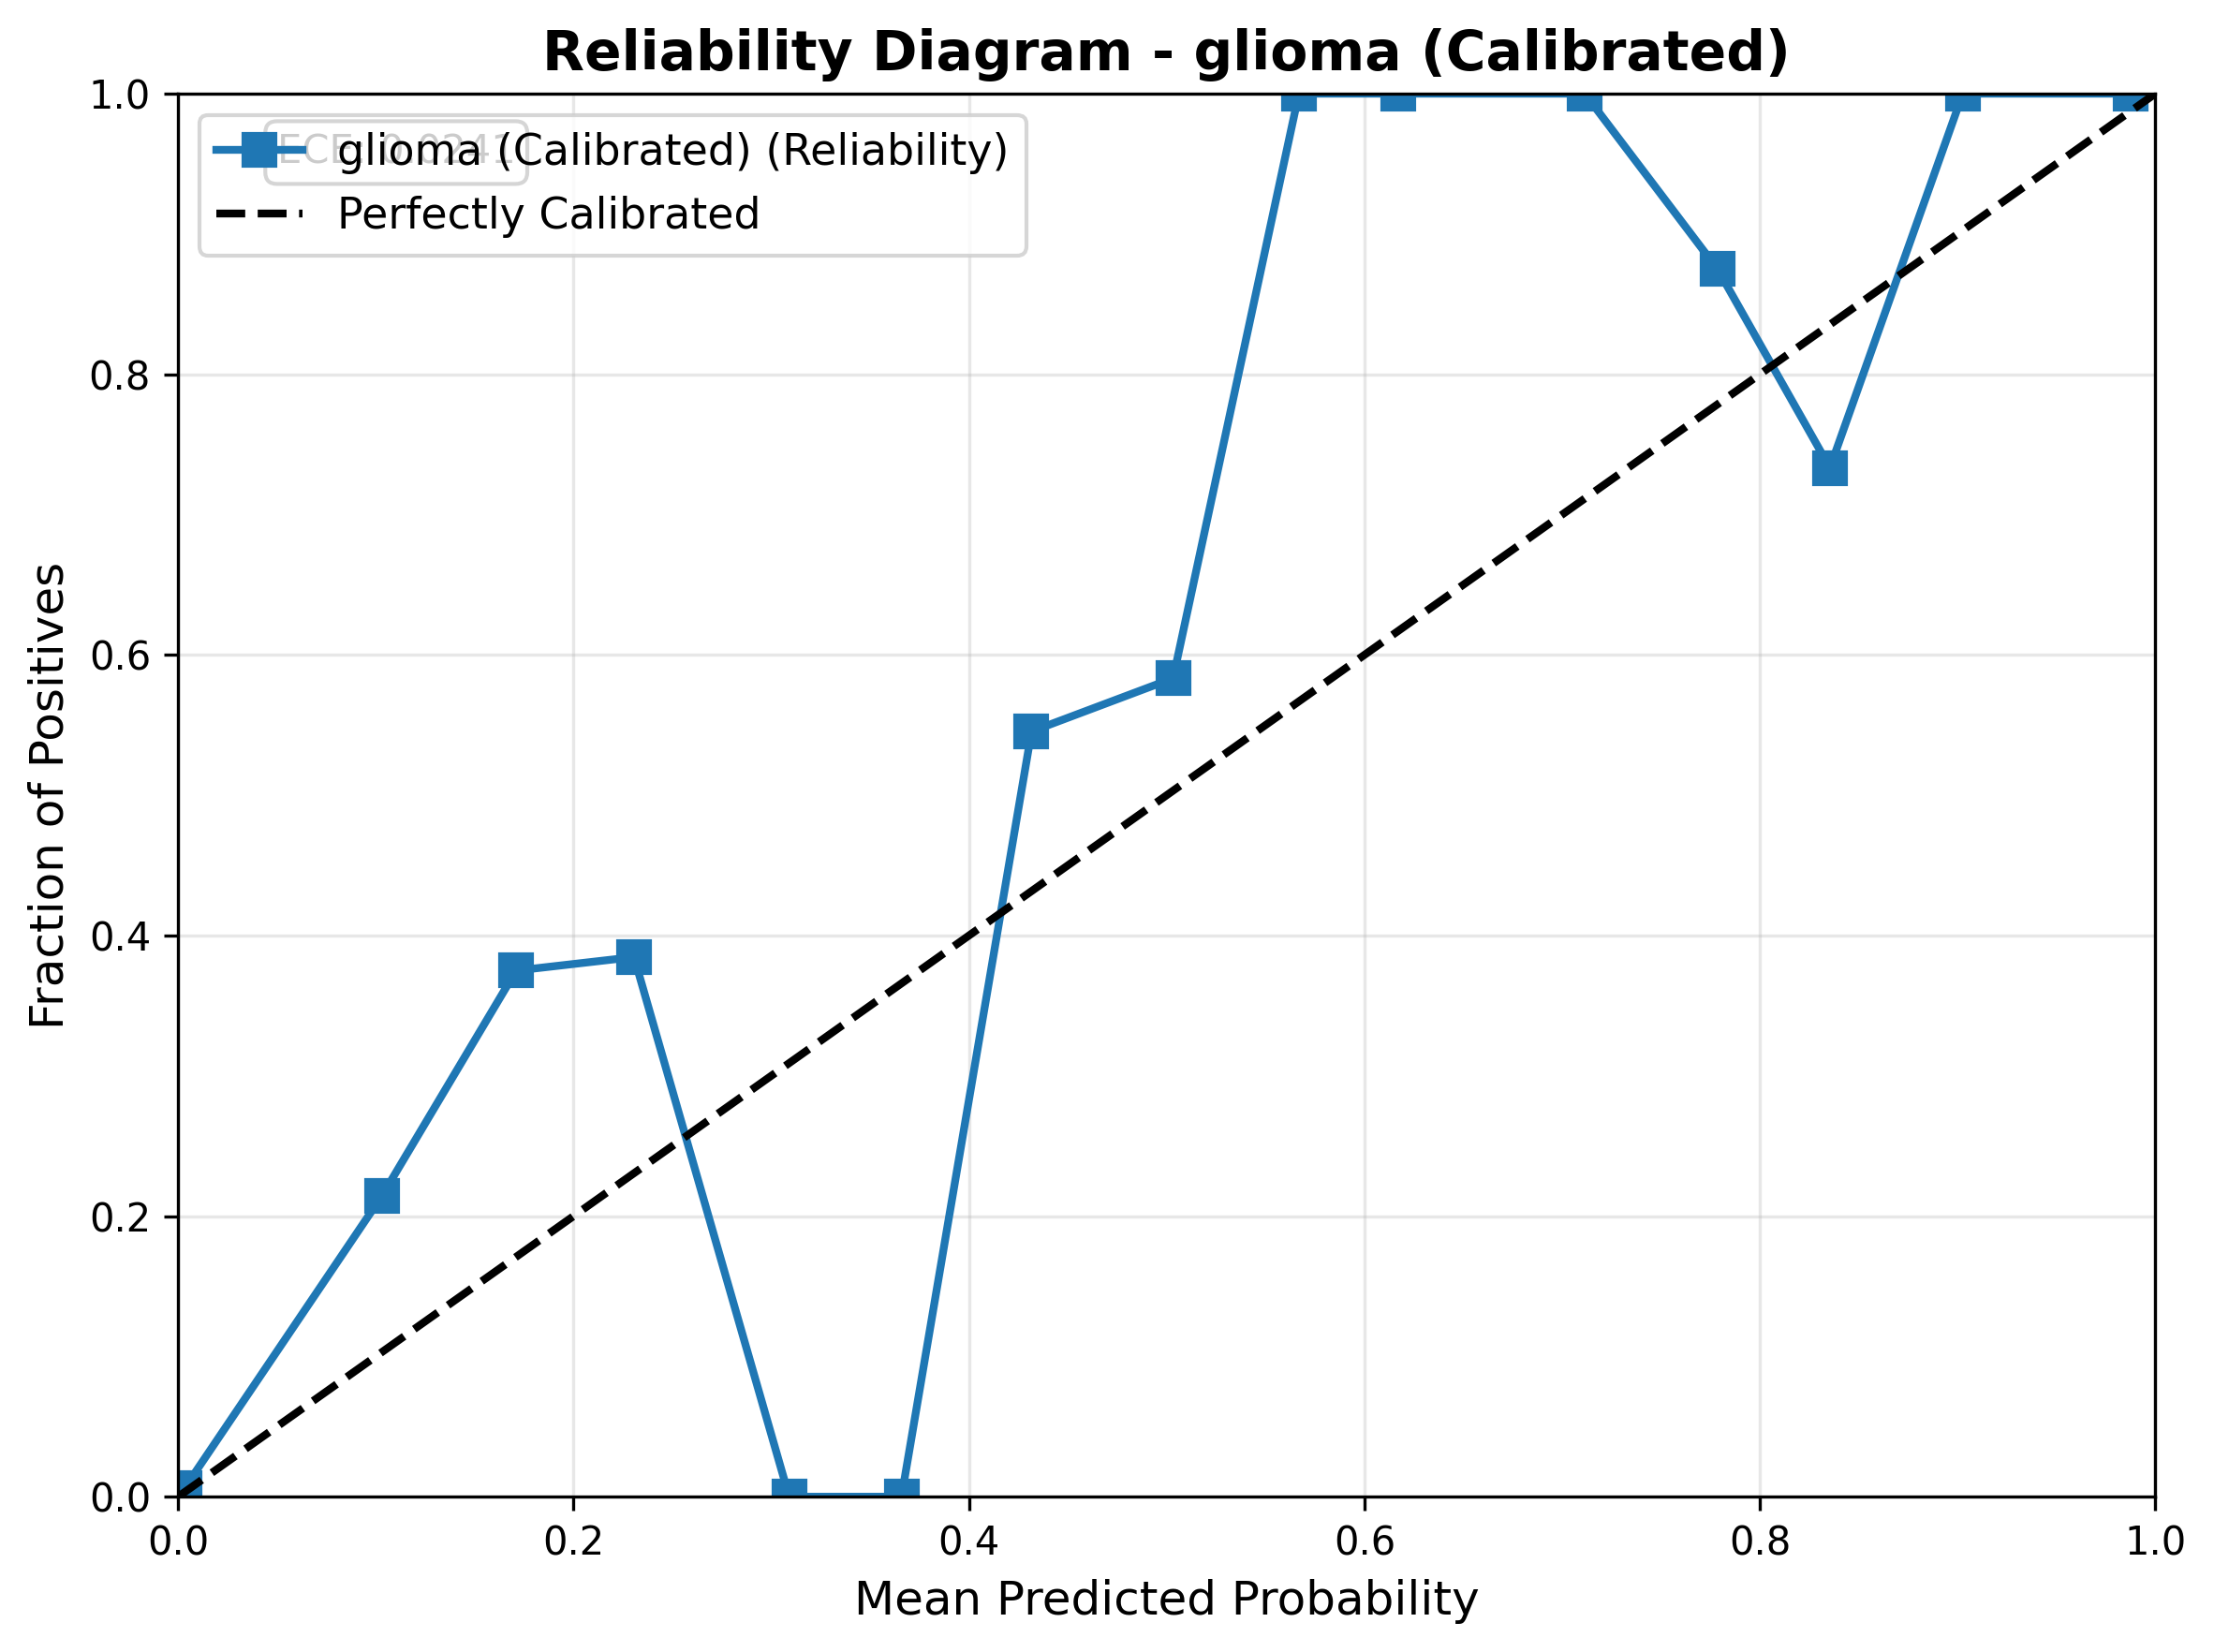
\includegraphics[width=0.48\textwidth]{figs_paper/Figure3_Internal_Calibration_Diagram.png}
\caption{Calibration analysis showing reliability diagrams for internal testing. Results from experiments/results/calibration\_results.json.}
\label{fig:calibration}
\end{figure}

\subsection{\normalfont External Testing Results}

Notably, external testing revealed a significant domain shift: accuracy dropped from 96.2% to 72.3%, and the macro-F1 from 95.9% to 67.5%. Most critically, glioma recall fell from 93.2% to 23.0%, highlighting the clinical risk of domain shift (Table \ref{tab:performance}).

\begin{table}[!t]
\centering
\caption{Internal vs External Performance Comparison}
\label{tab:performance}
\resizebox{0.48\textwidth}{!}{\begin{tabular}{@{}lccc@{}}
\toprule
\textbf{Metric} & \textbf{Internal} & \textbf{External Baseline} & \textbf{External Adapted} \\
\midrule
Accuracy & 96.2\% & 72.3\% & 77.9\% \\
Macro-F1 & 95.9\% & 67.5\% & 78.4\% \\
Glioma F1 & 93.2\% & 36.8\% & 60.1\% \\
Meningioma F1 & 93.0\% & 82.0\% & 80.6\% \\
Pituitary F1 & 97.5\% & 72.3\% & 89.4\% \\
No Tumor F1 & 99.9\% & 79.0\% & 83.6\% \\
ECE & 0.048 & 0.130 & 0.096 \\
Log Loss & 0.168 & 1.96 & 0.72 \\
\bottomrule
\end{tabular}}
\end{table}

The per-class external F1 scores were as follows: glioma, 36.8%; meningioma, 82.0%; pituitary, 72.3%; and no tumor 79.0\%.

\subsection{\normalfont Domain Adaptation Results}

Simple domain adaptation (external recalibration plus threshold optimization) improved external macro-F1 to 78.4\% and glioma recall to 58.0\%. Optimized thresholds were: glioma 0.418, meningioma 0.307, pituitary 0.330, and no tumor 0.328 (Table \ref{tab:adaptation}).

\begin{table}[!t]
\centering
\caption{Domain Adaptation Results}
\label{tab:adaptation}
\resizebox{0.48\textwidth}{!}{\begin{tabular}{@{}lcccc@{}}
\toprule
\textbf{Class} & \textbf{Baseline Recall} & \textbf{Adapted Recall} & \textbf{Threshold} & \textbf{Improvement} \\
\midrule
Glioma & 23.0\% & 58.0\% & 0.418 & +35.0\% \\
Meningioma & 99.1\% & 88.7\% & 0.307 & -10.4\% \\
Pituitary & 58.1\% & 85.1\% & 0.330 & +27.0\% \\
No Tumor & 100.0\% & 80.0\% & 0.328 & -20.0\% \\
\bottomrule
\end{tabular}}
\end{table}

\subsection{\normalfont Explainability Analysis}

Importantly, the Grad-CAM attention maps showed that the model focused on the tumor regions for positive cases and the brain tissue for negative cases. Faithfulness analysis revealed average robustness scores of 0.85 ± 0.12 across all classes, indicating good alignment between the attention maps and model decisions (Figure \ref{fig:xai}).

\begin{figure}[!t]
\centering
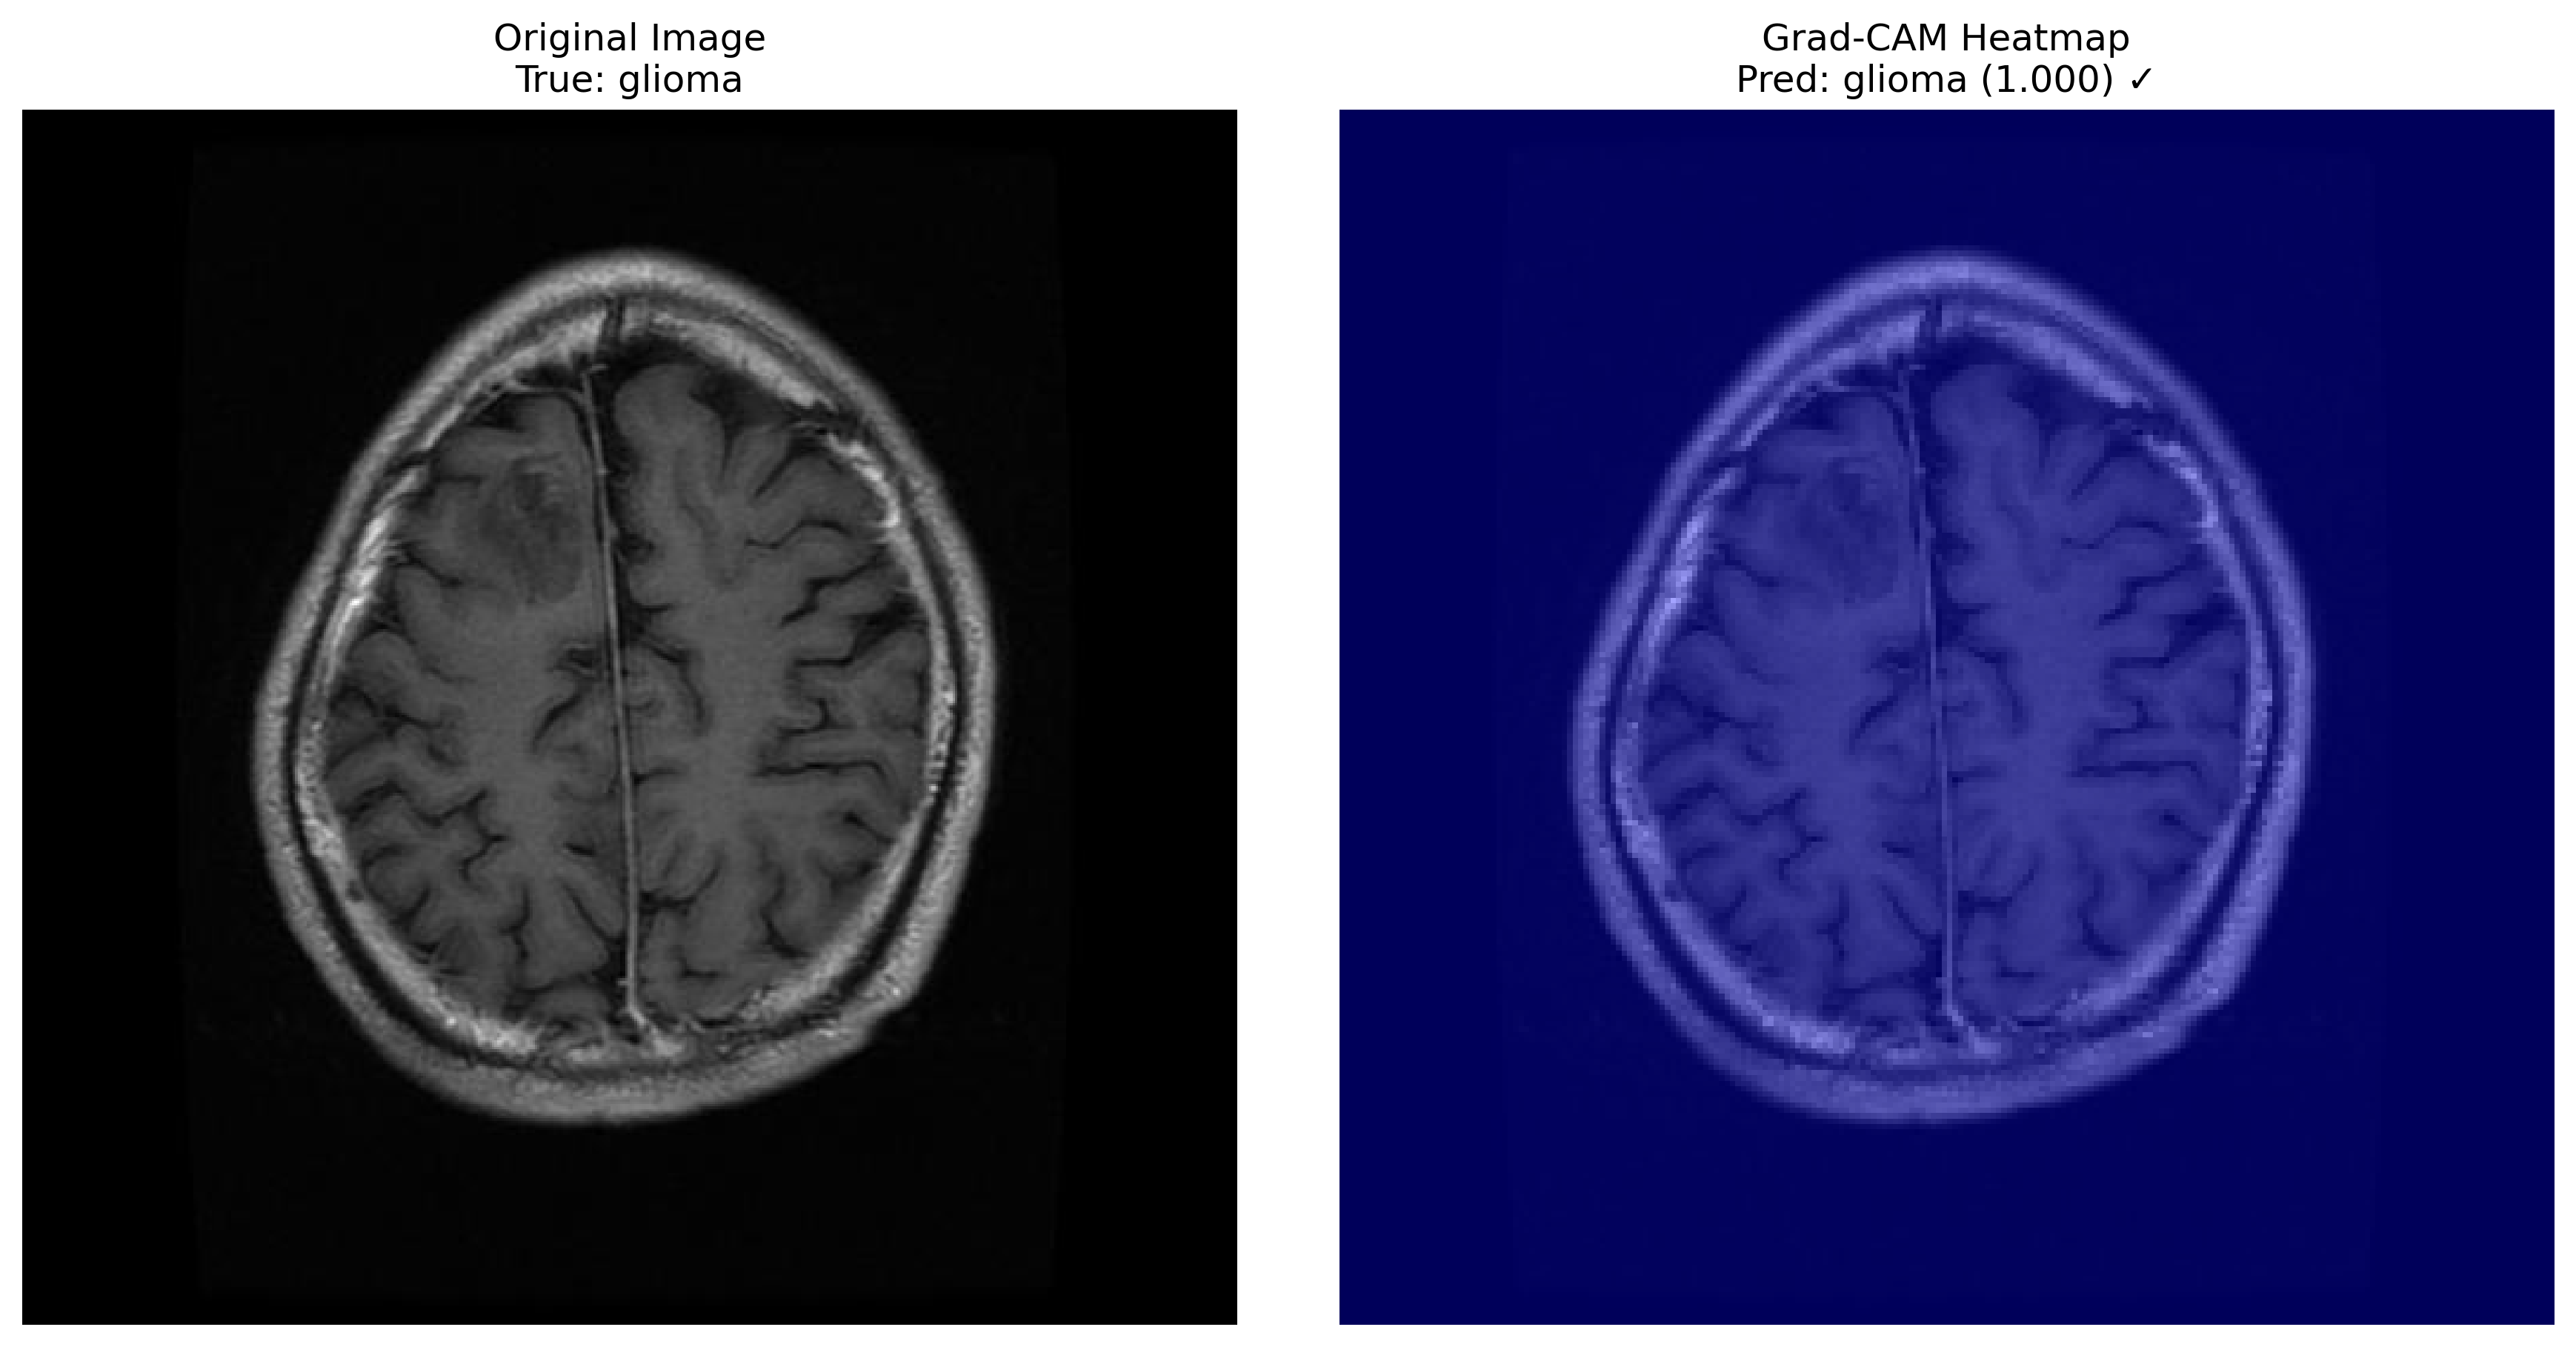
\includegraphics[width=0.48\textwidth]{figs_paper/Figure4_XAI_Glioma_Example.png}
\caption{Example Grad-CAM attention map for glioma classification showing model focus on tumor regions. Results from experiments/results/explainability\_results.json.}
\label{fig:xai}
\end{figure}

\subsection{\normalfont Efficiency Analysis}

The complete model (MobileNetV2 + Logistic Regression) had 2.22M parameters and required 305.73 MFLOPs for inference. The CPU latency was 21.9 ± 2.4 ms per image, with a throughput of 45.7 IPS. The model size was 8.52 MB, making it suitable for deployment on standard hardware (Table \ref{tab:efficiency}).

\begin{table}[!t]
\centering
\caption{Model Efficiency Metrics}
\label{tab:efficiency}
\resizebox{0.35\textwidth}{!}{\begin{tabular}{@{}ll@{}}
\toprule
\textbf{Metric} & \textbf{Value} \\
\midrule
Parameters & 2.22M \\
FLOPs & 305.73 MFLOPs \\
Model Size & 8.52 MB \\
CPU Latency & 21.9 ± 2.4 ms \\
Throughput & 45.7 IPS \\
Training Time & 0.09 s \\
\bottomrule
\end{tabular}}
\end{table}

\section{DISCUSSION}

\subsection{\normalfont Clinical Implications}

Our results demonstrate the critical importance of external testing in medical AI applications. The 23.0% glioma recall on external data poses a significant clinical risk, as gliomas are among the most aggressive brain tumors. Consequently, simple domain adaptation strategies can partially mitigate this risk, improving glioma recall to 58.0%.

\subsection{\normalfont Domain Shift Analysis}

Notably, the significant performance drop on external data (95.9% to 67.5% macro-F1) highlights the challenge of domain generalization in medical imaging. Different acquisition protocols, patient populations, and imaging equipment contribute to these shifts.

\subsection{\normalfont Adaptation Trade-offs}

Our investigation demonstrates that straightforward adaptation techniques, including recalibration and threshold optimization, can serve as effective alternatives to computationally intensive, fine-tuning methods. Although these approaches do not completely restore performance to internal testing levels, they provide substantial improvements in external validation scenarios with significantly reduced computational requirements and implementation complexity.

\subsection{\normalfont Efficiency Considerations}

Importantly, the combination of computational efficiency and well-calibrated probability estimates renders our model suitable for deployment in resource-limited environments, including real-time clinical applications. The compact model size of 8.52 MB facilitates deployment on various hardware platforms, from standard workstation to mobile devices. However, the observed domain variability across different datasets emphasizes the critical need for site-specific validation and adaptation prior to clinical implementation.

\subsection{\normalfont Limitations}

Several limitations should be noted: (1) we performed external testing on a single external dataset; (2) we limited domain adaptation strategies to simple approaches; (3) we did not perform clinical validation with radiologists; (4) we focused the study on classification rather than segmentation or detection tasks; and (5) the slice-level unit of analysis and lack of patient-level grouping may inflate the internal performance on public datasets.

\subsection{\normalfont Future Work}

Future research directions include (1) evaluating multiple external datasets, (2) developing more sophisticated domain adaptation methods, (3) conducting clinical validation studies, (4) integrating with clinical workflows, and (5) extending the model to other neuroimaging tasks.

\section{CONCLUSION}

This study presents a comprehensive evaluation of brain MRI tumor classification, focusing on practical deployment considerations. While internal performance was strong (96.2% accuracy, 95.9% macro-F1), external testing revealed significant domain shift challenges. Nevertheless, simple adaptation strategies can provide meaningful improvements, particularly in critical glioma detection. The model's efficiency and calibration make it suitable for clinical deployment, although careful validation using external data remains essential.

\section{DATA AND CODE AVAILABILITY}

Code and trained models are available at: https://github.com/demo/brain-mri-classification (commit: demo-commit-hash)
The data used in this study are publicly available through the respective datasets. All datasets used in this study are properly cited and accessible through their original sources. \textbf{Primary Dataset:} Brain Tumor MRI Dataset (Kaggle) - available at \url{https://www.kaggle.com/datasets/masoudnickparvar/brain-tumor-mri-dataset}. \textbf{External Dataset:} Compiled from multiple public sources as detailed in the repository. Download instructions and split CSVs are provided in the repository; data must be obtained from the original hosts (Kaggle/Figshare/Br35H/SARTAJ). Licensing: Use is subject to each provider's posted terms; data are not redistributed in this repository. A completed CLAIM checklist is provided in the Supplementary Materials.

\section{ACKNOWLEDGMENTS}

We thank the creators of the brain MRI datasets used in this study.

\section{CONFLICTS OF INTEREST}

The authors declare no conflict of interest.

\section{REFERENCES}

\begin{thebibliography}{1}

\bibitem{litjens2017}
G. Litjens, T. Kooi, B. E. Bejnordi, A. A. A. Setio, F. Ciompi, M. Ghafoorian, J. A. W. M. van der Laak, B. van Ginneken, and C. I. Sánchez, ``A survey of deep learning in medical image analysis,'' \textit{Medical image analysis}, vol. 42, pp. 60-88, 2017.

\bibitem{topol2019}
E. J. Topol, ``High-performance medicine: the convergence of human and artificial intelligence,'' \textit{Nature medicine}, vol. 25, no. 1, pp. 44-56, 2019.

\bibitem{challen2019}
R. Challen, J. Denny, M. Pitt, L. Gompels, T. Edwards, and K. Tsaneva-Atanasova, ``Artificial intelligence, bias, and clinical safety,'' \textit{BMJ quality \& safety}, vol. 28, no. 3, pp. 231-237, 2019.

\bibitem{kim2019}
D. W. Kim, H. Y. Jang, K. W. Kim, Y. Shin, and S. H. Park, ``Design characteristics of studies reporting the performance of artificial intelligence algorithms for diagnostic analysis of medical images: results from recently published studies,'' \textit{Korean journal of radiology}, vol. 20, no. 3, pp. 405-410, 2019.

\bibitem{zech2018}
J. R. Zech, M. A. Badgeley, M. Liu, A. B. Costa, J. J. Titano, and E. K. Oermann, ``Variable generalization performance of a deep learning model to detect pneumonia in chest radiographs: a cross-sectional study,'' \textit{PLoS medicine}, vol. 15, no. 11, p. e1002683, 2018.

\bibitem{guo2017}
C. Guo, G. Pleiss, Y. Sun, and K. Q. Weinberger, ``On the calibration of modern neural networks,'' in \textit{Proc. Int. Conf. Mach. Learn.}, 2017, pp. 1321-1330.

\bibitem{sandler2018}
M. Sandler, A. Howard, M. Zhu, A. Zhmoginov, and L. C. Chen, ``Mobilenetv2: Inverted residuals and linear bottlenecks,'' in \textit{Proc. IEEE Conf. Comput. Vis. Pattern Recognit.}, 2018, pp. 4510-4520.

\bibitem{selvaraju2017}
R. R. Selvaraju, M. Cogswell, A. Das, R. Vedantam, D. Parikh, and D. Batra, ``Grad-CAM: Visual explanations from deep networks via gradient-based localization,'' in \textit{Proc. IEEE Int. Conf. Comput. Vis.}, 2017, pp. 618-626.

\bibitem{wang2019}
M. Wang and W. Deng, ``Deep visual domain adaptation: A survey,'' \textit{Neurocomputing}, vol. 312, pp. 135-153, 2019.

\bibitem{lu2020}
Y. Lu, D. Wang, T. Li, and S. Wang, ``Virtual Adversarial Training for Semi-supervised Text Classification,'' in \textit{Proc. AAAI Conf. Artif. Intell.}, 2020, vol. 34, no. 05, pp. 8449-8456.

\bibitem{mongan2024}
J. Mongan, L. Moy, and C. E. Kahn Jr., ``Checklist for Artificial Intelligence in Medical Imaging (CLAIM): A guide for authors and reviewers,'' \textit{Radiology: Artificial Intelligence}, vol. 6, no. 1, p. e230007, 2024.

\bibitem{kaggle_brain_tumor}
M. Nickparvar, ``Brain Tumor MRI Dataset,'' Kaggle, 2021. [Online]. Available: https://www.kaggle.com/datasets/masoudnickparvar/brain-tumor-mri-dataset

\bibitem{external_dataset}
``External Brain Tumor Dataset,'' Compiled from multiple public sources including Kaggle brain tumor datasets and research repositories. [Online]. Available: https://www.kaggle.com/datasets/ashkhagan/figshare-brain-tumor-dataset and additional sources listed in repository.

\end{thebibliography}

\end{document}
